

\begin{frame}
\frametitle{The Upper Confidence Bound (UCB) Approach}
\begin{itemize}
\item<1-> Since there is an initial uncertainty in the estimated mean ($\hat{r}_i$) introduce a confidence interval term $c_i$.
\item<2-> $c_i$ ensures that the arm $i$ is properly explored and is gradually reduced with time as one pulls the arm $i$ more.
\item<3-> At every timestep pull arm that has the maximum value of $\hat{r}_i + c_i$ and this will ensure that proper exploration is done. 
\end{itemize}
\end{frame}

\begin{frame}
\frametitle{The UCB Approach}
\begin{figure}
%\caption{UCB Intuition}
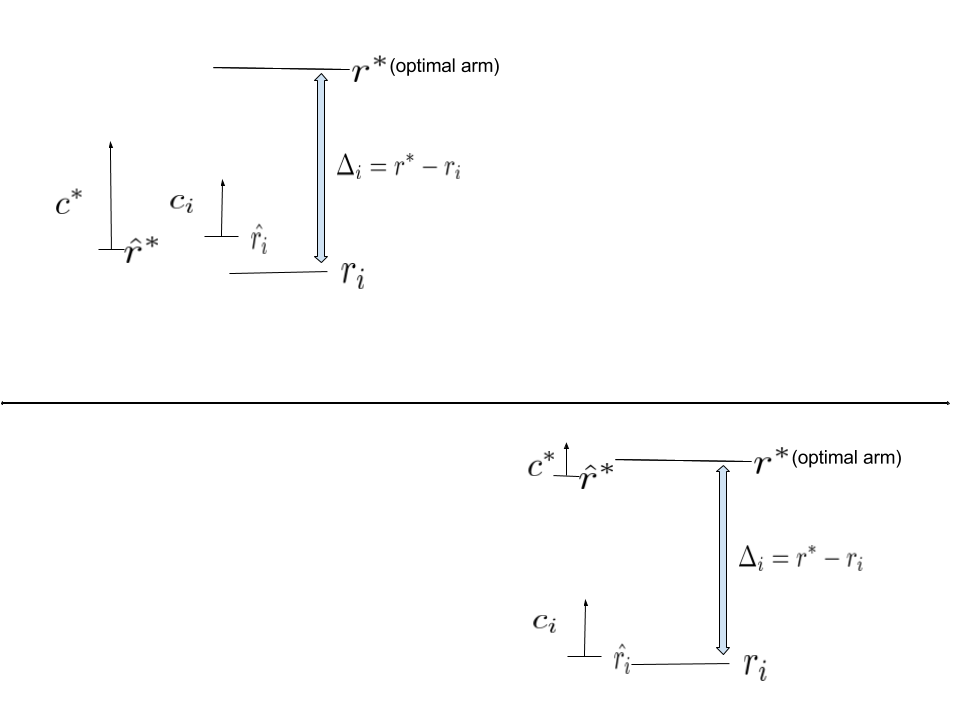
\includegraphics[scale=0.3]{img/UCB_Drawing.png}
\end{figure}
\end{frame}


%\begin{frame}
%\frametitle{Previous Works (Pure Exploration)}
%\begin{itemize}
%\item<1-> The TBP problem also falls within the larger area called the Pure Exploration problem.
%\item<2-> In pure exploration problems the learner has to output a set of recommendations either with high confidence (fixed confidence) or after a specified number of rounds (fixed budget).
%\item<3-> Our considered TBP is a fixed budget pure exploration problem.
%\item<4-> Both APT and AugUCB reuses several ideas from Pure exploration problem. 
%\end{itemize}
%\end{frame}
%
%\begin{frame}
%\frametitle{Previous Works (Diagram)}
%\centering
%\begin{figure}
%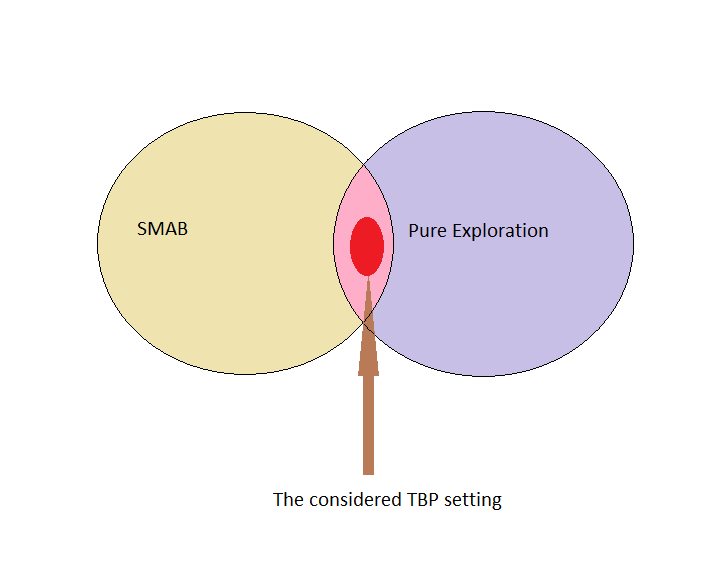
\includegraphics[scale=0.3]{img/Settings2.png}
%\caption{TBP place within SMAB and Pure exploration}
%\end{figure}
%\end{frame}

%\begin{frame}
%\frametitle{Approach of UCB-Improved (UCB-Imp)}
%\begin{itemize}
%\item<1-> There is a strong relation between UCB-Imp \cite{auer2010ucb} and AugUCB where the former is used to find \emph{a single optimal arm as quickly as possible}.
%\item<2-> The basic idea of UCB-Improved is to divide the horizon into phases or rounds and initialize parameters.
%\item<3-> Pull all surviving arms equal number of times during a round.
%\item<4-> At the end of the round eliminate some sub-optimal arms (as judged by learner) based on elimination criteria.
%\item<5-> Reset parameters and proceed to next round.
%\end{itemize}
%\end{frame}
%
%\begin{frame}
%\frametitle{UCB-Improved (\cite{auer2010ucb})}
%\begin{algorithm}[H]
%\caption{UCB-Improved}
%\small
%\begin{algorithmic}[1]
%\State {\bf Input:} Time horizon $T$
%\State {\bf Initialization:} Set $B_{0}:=A$ and ${\epsilon}_{0}:=1$.
%\For{$m=0,1,..\big \lfloor \dfrac{1}{2}\log_{2} \dfrac{T}{e}\big\rfloor$}	
%\State Pull each arm in $B_m$, $n_{m}=\bigg\lceil\dfrac{2\log{( T{\epsilon}_{m}^{2})}}{{\epsilon}_{m}}\bigg\rceil$ number of times.
%%so that the total  it has been pulled is
%\ArmElim
%\State For each $i \in B_{m}$, delete arm ${i}$ from $B_{m}$ if,
%\begin{align*}
%\hat{r}_{i} + \sqrt{\dfrac{\log{(T{\epsilon}_{m}^{2})}}{2 n_{m}}}  < \max_{{j}\in B_{m}}\bigg\lbrace\hat{r}_{j} -\sqrt{\dfrac{\log{( T{\epsilon}_{m}^{2})}}{2 n_{m}}} \bigg\rbrace
%\end{align*}
%\EndArmElim
%%\ResParam
%\State Set ${\epsilon}_{m+1}:=\dfrac{{\epsilon}_{m}}{2}$, Set $B_{m+1}:=B_{m}$
%%\EndResParam
%\State Stop if $|B_{m}|=1$ and pull ${i}\in B_{m}$ till $T$ is reached.
%\EndFor
%\end{algorithmic}
%\end{algorithm}
%\end{frame}

\begin{frame}
\frametitle{Approach of UCB-Improved (UCB-Imp)}
\begin{figure}
%\caption{UCB Imp Approach}
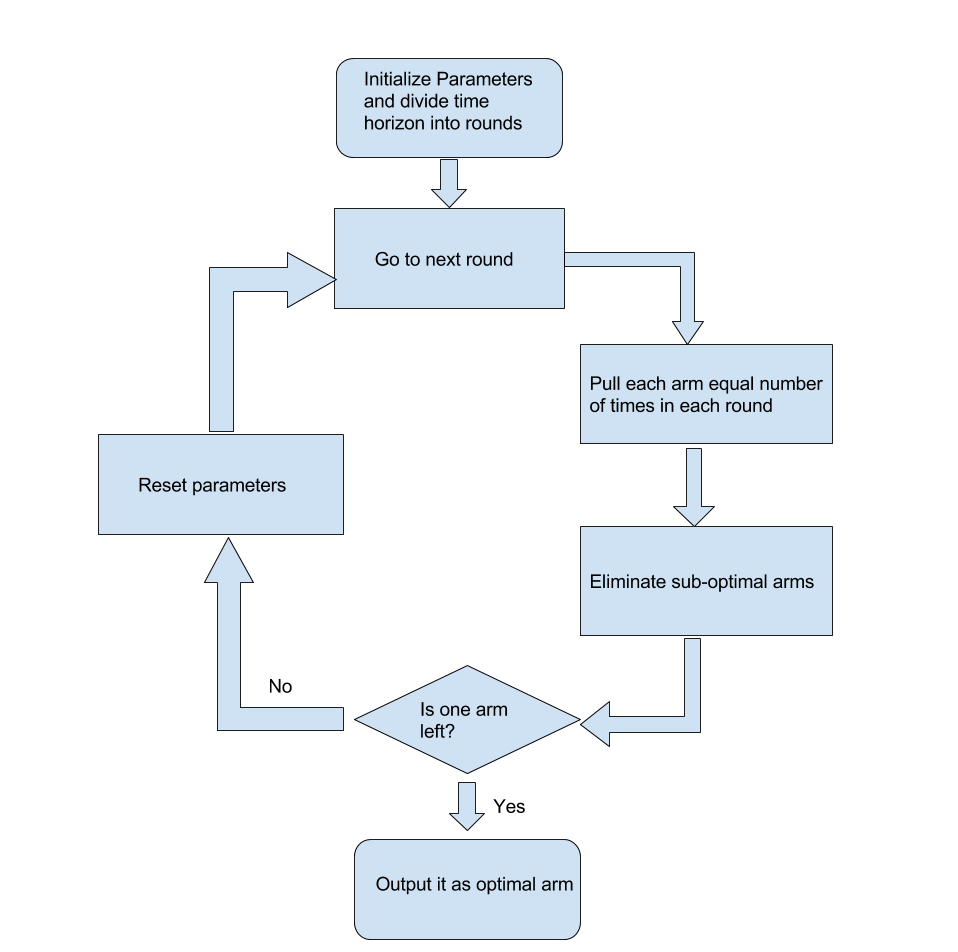
\includegraphics[scale=0.25]{img/Ucb-Imp.png}
\end{figure}
\end{frame}



\begin{frame}
\frametitle{Intuition of UCB-Improved (UCB-Imp)}
\begin{figure}
%\caption{UCB Imp Intuition}
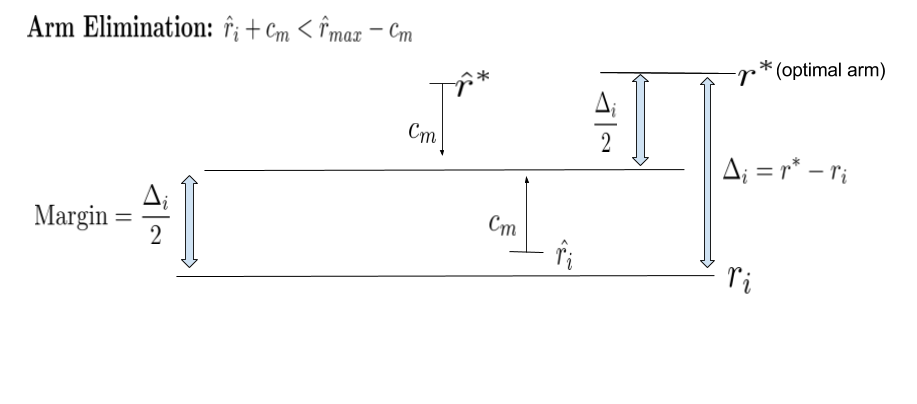
\includegraphics[scale=0.3]{img/Ucb_Imp_intuition.png}
\end{figure}
\end{frame}


\begin{frame}
\frametitle{APT Approach}
\begin{itemize}
\item<1-> The Anytime Parameter Free (APT) [{Locatelli et al. (2016)}] algorithm was proposed for TBP setting in ICML 2016. 
\item<2-> This algorithm uses only mean estimation to find the $S_{\tau}$. 
\item<3-> Theoretically they proved this algorithm to be almost optimal when only mean estimation is used as a metric of comparison.
\item<4-> Empirically it outperformed other state-of-the-art algorithms which were modified to perform in the TBP setting.  
\end{itemize}
\end{frame}

\begin{frame}
\frametitle{APT Algorithm}
\begin{algorithm}[H]
\caption{APT}
\begin{algorithmic}
\State {\bf Input:} Time horizon $T$, threshold $\tau$, tolerance factor $\epsilon\geq 0$
\State Pull each arm once
\vspace{-3mm}
\State \For{$t=K+1,..,T$}
\State Pull arm $j\in\argmin_{i\in A}\Big\lbrace \left(|\hat{r}_{i} - \tau | + \epsilon\right)\sqrt{n_i}\Big\rbrace$ and observe the reward for arm $j$.
\EndFor
\State \textbf{Output:} $\hat{S}_{\tau}=\lbrace i: \hat{r}_{i}\geq \tau \rbrace$.
\end{algorithmic}
\end{algorithm}
\end{frame}


\begin{frame}
\frametitle{Intuition of APT}
\begin{figure}
%\caption{APT Intuition}
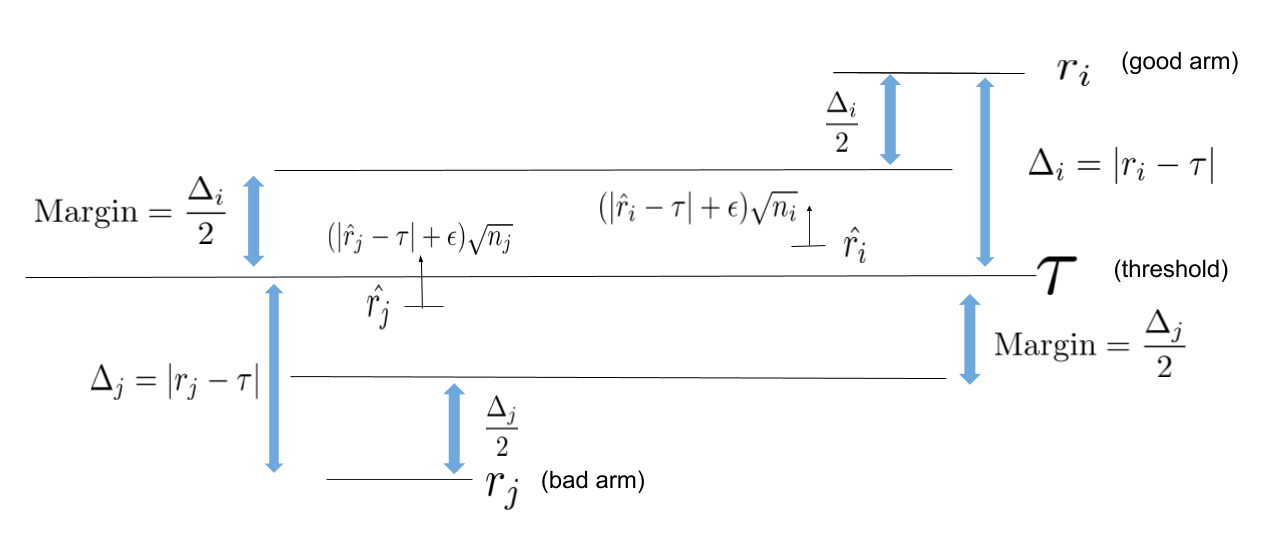
\includegraphics[scale=0.278]{img/APT_intuition.png}
\end{figure}
\end{frame}





%\begin{frame}
%\frametitle{Some technical details of UCB-Improved}
%\begin{itemize}
%\item<1-> We do not know the true means $r_i ,\forall i\in A$ of the distributions so we estimate it by the ${\epsilon}$ by initializing it from $1$.
%\item<2-> All rewards are assume to be bounded between $[0,1]$ and so $\Delta_{i} = (r^* - r_i)\in [0,1],\forall i\in A$ as well.
%\item<3-> UCB-Improved has fixed confidence interval  $c_{m}=\sqrt{\dfrac{\log{(T{\epsilon}_{m}^{2})}}{2 n_{m}}}$ for all arms in a particular round.
%\item<4-> $c_m$ ensures that whenever ${\epsilon}_{m}<\dfrac{\Delta_i}{2}$ in the $m$-th round, the arm $i$ gets eliminated.
%\end{itemize}
%\end{frame}